\section{Deep Reinforcement Learning}
In contrast to the manually developed algorithm, a Deep Q-learning based search algorithm was also developed. The agents is trained in using the simple simulator to search the map. Reinforcement learning suits this problem well as coverage can serve as a {\color{red} good} reward function. Traditional Q-learning methods store a table of discrete state-action pairs and their expected reward in memory {\color{red}[SOURCE]}. This table is called a Q-table. However, in real world applications state is often continuous, which creates the need to {\color{red} disoretize} the agent state. Another problem is that the size of the Q-table grows with the state space. Neural networks solve both of these problems. The Q-table can be approximated by using a neural network and then used to pick an action given a state.

A lot of considerations must be made when designing the network. First, the number of neurons in each layer must be chosen. Second, the activation function must be chosen. Third, the learning rate must be chosen. Fourth, the network must be trained. Fifth, the network must be tested. Sixth, the network must be optimized. Seventh, the network must be deployed.

\subsection{Network}
The general idea of a neural network is to have a set of layers. Each layer has a number of neurons. The neurons are connected to each other. The output of the last layer is the action that the agent should take. The input to the network is the state of the agent.

% TODO: Write how our network and activation function works (maybe in each of the models or only one?)

\subsection{Reward}
Reinforcement learning relies on a reward function. The reward function is used to determine how good a state is. In the ideal world the model would be able to perfectly predict the best action to take in a given state. However, in real world applications, the model is not perfect. The reward function is used to punish the agent for making mistakes. A good reward function will encourage the agent to make the correct decisions.

% TODO: Write how our reward function works (maybe in each of the models or only one?)

\subsection{Training}
In order to train the network, the agent must be able to learn. This is done by the agent taking actions and receiving rewards. The agent then updates its network to make better decisions in the future. The agent is trained by running the simulation for a number of episodes. 
Each episode is a single run of the simulation and is stopped if no progress is made or the whole map is covered.

\subsubsection{Generating Training Environments}
As to not overfit the network, it must be trained on many different environments. A simple program was created to generate worlds populated by line and circle obstacles.

\def\w{0.31\textwidth}
\begin{figure}[H]
    \begin{subfigure}{\w}
        \makebox(\textwidth, \textwidth)[\textwidth]{
            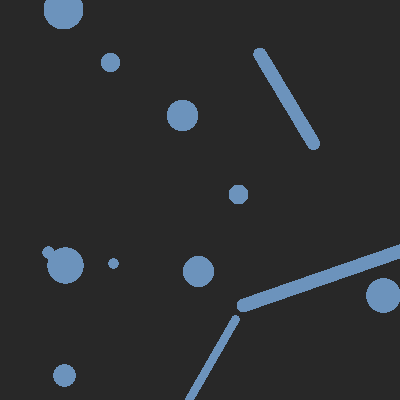
\includegraphics[width=\linewidth]{figures/generated-worlds/world_0.png}
        }
    \end{subfigure}
    \hspace*{\fill}
    \begin{subfigure}{\w}
        \makebox(\textwidth, \textwidth)[\textwidth]{
            
\includegraphics[width=\linewidth]{figures/generated-worlds/world_1.png}
        }
    \end{subfigure}
    \hspace*{\fill}
    \begin{subfigure}{\w}
        \makebox(\textwidth, \textwidth)[\textwidth]{
            
\includegraphics[width=\linewidth]{figures/generated-worlds/world_2.png}
        }
    \end{subfigure}

    \vspace{4mm}

    \begin{subfigure}{\w}
        \makebox(\textwidth, \textwidth)[\textwidth]{
            
\includegraphics[width=\linewidth]{figures/generated-worlds/world_3.png}
        }
    \end{subfigure}
    \hspace*{\fill}
    \begin{subfigure}{\w}
        \makebox(\textwidth, \textwidth)[\textwidth]{
            
\includegraphics[width=\linewidth]{figures/generated-worlds/world_4.png}
        }
    \end{subfigure}
    \hspace*{\fill}
    \begin{subfigure}{\w}
        \makebox(\textwidth, \textwidth)[\textwidth]{
            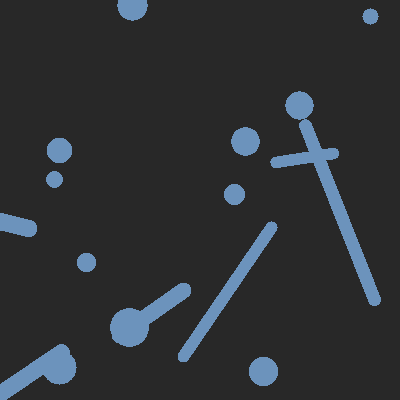
\includegraphics[width=\linewidth]{figures/generated-worlds/world_5.png}
        }
    \end{subfigure}
    \caption{Examples of generated environments} \label{fig:generated-enviornments}
\end{figure}

\end{document}
